\documentclass[11pt]{article}
\usepackage[a4paper,margin=25mm]{geometry}
\usepackage[T1]{fontenc}
\usepackage[utf8]{inputenc}
\usepackage{lmodern}
\usepackage{graphicx}
\usepackage{booktabs}
\usepackage{amsmath}
\usepackage{xspace}
\usepackage{hyperref}
\renewcommand{\topfraction}{0.9}
\renewcommand{\bottomfraction}{0.9}
\renewcommand{\textfraction}{0.1}
\newcommand{\code}[1]{\texttt{#1}}
\newcommand{\us}{\textmu s\xspace}
\newcommand{\Na}{\ensuremath{{}^{22}\mathrm{Na}}\xspace}

\title{The BGO temperature scan of 2 October 2026:\\ the data, the detector and the single photoelectron}
\author{J.\,J.~Gómez-Cadenas}
\date{14 October 2026}

\begin{document}
\maketitle

\begin{abstract}
A BGO crystal read out by 64 SiPMs was operated in a cryostat between 128 and
197~K, with the SiPM bias changed with the temperature, and irradiated with
a \Na source. The purpose of the measurement is the light yield and the
energy resolution of the crystal at 511~keV as a function of temperature and
SiPM overvoltage. This note documents what was learned about the data and
the detector before that analysis: the conditions of each run, the
overvoltage at which the SiPMs operated, the behaviour of the trigger and
the readout, what the events look like, the state of the 64 channels, and
the single-photoelectron response, which gives the gain of each channel.
The analysis itself is the subject of a second note.
\end{abstract}

\section{The data set}
\label{sec:data}

The detector is a BGO crystal of $48 \times 48$~mm$^2$ and 20~mm thickness,
wrapped in Teflon on all faces but one. That face is read out by 64
Hamamatsu S14160-6050HS SiPMs of $6 \times 6$~mm$^2$, arranged in an $8
\times 8$ matrix at 6~mm pitch that covers the face exactly. The SiPMs are
mounted in four $4 \times 4$ tiles; the pitch is 6.2~mm inside a tile and
6.4~mm across the gap between tiles. The digitizer channel of each SiPM and
its position on the face are given in \code{src/channel\_map.csv}: channel
$c$ sits at column $c \bmod 8$ and row $c \div 8$, $x$ growing with the
column from $-21.8$ to $+21.8$~mm and $y$ decreasing with the row from
$+21.8$ to $-21.8$~mm.

\begin{figure}[tbp]
\centering
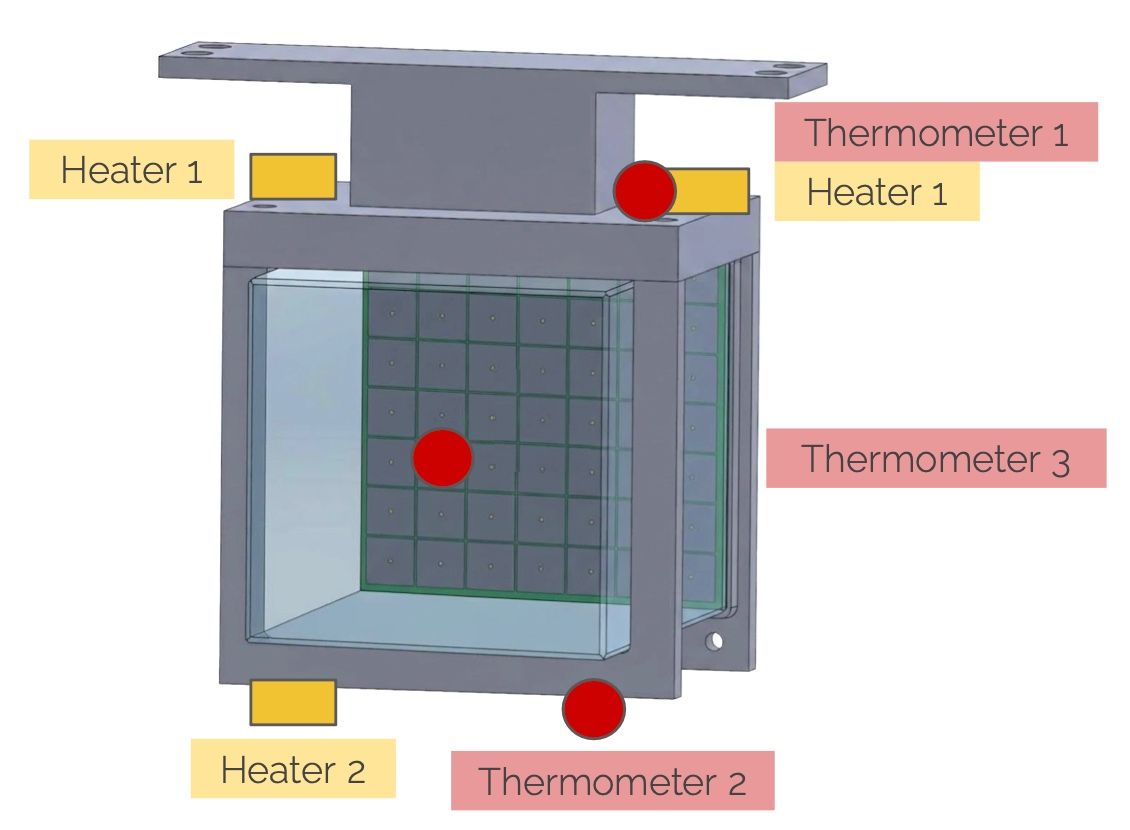
\includegraphics[width=0.6\linewidth]{figs/thermometers.jpg}
\caption{The mechanics, schematic (the array is drawn $6 \times 6$; the real
one is $8 \times 8$). The crystal hangs inside an aluminium frame; the SiPM
board closes its back. Two heaters warm the frame, at the top plate and at
the bottom. Thermometer 1 is on the top plate, thermometer 2 at the bottom
of the frame, thermometer 3 at the centre of the back face, between the
Teflon and the SiPM array.}
\label{fig:thermo}
\end{figure}

The crystal hangs inside an aluminium frame (Figure~\ref{fig:thermo}),
which is cooled in a cryostat and warmed by two resistors, one on the top
plate and one at the bottom of the frame. There is no temperature
regulation: the heaters set the temperature and three thermometers measure
it, T1 on the top plate, T2 at the bottom of the frame, and T3 at the
centre of the back face of the crystal, between the Teflon and the SiPM
array. The source is \Na, placed 3~cm from the face, on its axis. It emits
two 511~keV gammas back to back, of which only one can reach the crystal,
and a 1275~keV gamma. From 3~cm the source illuminates the whole crystal.

Twelve runs of 5000 events each were taken, at crystal temperatures from
128 to 197~K (Table~\ref{tab:runs}). Along the temperature scan the bias
was raised with the temperature, from 37 to 41~V in steps of 1~V, to keep
the overvoltage of the SiPMs nominally constant. Two bias scans were added
at the warm end: at about 185~K the bias was lowered from 40~V to 38.5~V in
steps of 0.5~V, and at about 196~K from 41~V to 39~V, each step a run of
5000 events. The runs are named after the crystal temperature, the bias and
the trigger threshold: \code{185K\_39d5V\_th19} is 185~K, 39.5~V, 19 ADC
counts.

\begin{table}[tbp]
\centering
\caption{The runs, in order of acquisition, with the three thermometer
readings in kelvin (from \code{temperatures.txt}), the SiPM bias and the
trigger threshold. The last column is the true trigger rate of the board,
from Section~\ref{sec:daq}.}
\label{tab:runs}
\begin{tabular}{l l r r r r r r}
\toprule
run & start & T1 & T2 & T3 & bias (V) & threshold & trigger rate \\
\midrule
128K\_37V\_th19   & 14:47 & 131.0 & 131.8 & 128.6 & 37.0 & 19 & 1.9 kHz \\
153K\_38V\_th19   & 14:54 & 161.6 & 157.5 & 153.1 & 38.0 & 19 & 20 kHz \\
164K\_39V\_th19   & 15:00 & 170.7 & 172.9 & 164.8 & 39.0 & 19 & 66 kHz \\
184K\_40V\_th19   & 15:13 & 180.7 & 190.1 & 184.8 & 40.0 & 19 & 132 kHz \\
185K\_39d5V\_th19 & 15:15 & 181.0 & 190.1 & 185.8 & 39.5 & 19 & 80 kHz \\
186K\_39V\_th19   & 15:16 & 181.2 & 190.2 & 186.6 & 39.0 & 19 & 43 kHz \\
187K\_38d5V\_th19 & 15:17 & 181.5 & 190.2 & 187.4 & 38.5 & 19 & 19 kHz \\
195K\_41V\_th20   & 15:28 & 183.7 & 205.0 & 195.8 & 41.0 & 20 & 225 kHz \\
196K\_40d5V\_th20 & 15:29 & 183.8 & 203.9 & 196.2 & 40.5 & 20 & 148 kHz \\
196K\_40V\_th20   & 15:30 & 183.9 & 203.1 & 196.6 & 40.0 & 20 & 97 kHz \\
196K\_39d5V\_th20 & 15:33 & 184.0 & 202.5 & 196.9 & 39.5 & 20 & 29 kHz \\
197K\_39V\_th20   & 15:35 & 184.1 & 201.9 & 197.3 & 39.0 & 20 & 2.7 kHz \\
\bottomrule
\end{tabular}
\end{table}

The temperatures were not stabilised; the runs were taken in a hurry,
each one about a minute after the previous one. The consequences are
visible in the table. Within each bias scan the crystal temperature T3
rises from run to run, from 184.8 to 187.4~K in the first and from 195.8 to
197.3~K in the second, while T2 is steady in the first and relaxing from an
overshoot in the second: the frame was at its temperature, and the crystal,
isolated by the Teflon, was still catching up. For the analysis each run
is taken at its measured T3, and a bias scan is not at one temperature but
spread over 1.5 to 2.6~K. The effect of that spread on the light yield is
a correction of the order of a percent, small against the effect of the
bias.

The frame also had a strong vertical gradient at the warm end: T1 and T2
differ by 9~K in the first bias scan and by about 20~K in the second,
bottom warmer. The SiPM board is mounted on the frame, so the SiPMs were
probably warmer than the crystal, somewhere between T3 and T2, and the
bottom rows possibly warmer than the top rows. This matters for the
overvoltage, which depends on the SiPM temperature, and we come back to it
in the next section.

\section{The SiPMs and their overvoltage}
\label{sec:sipm}

The S14160-6050HS is a 6~mm SiPM with 50~\textmu m pixels and a low breakdown
voltage. The datasheet gives, at 25~\textdegree C: breakdown voltage
$V_{\rm bd} = 38$~V, recommended operation at $V_{\rm bd} + 2.7$~V, a
temperature coefficient of the breakdown of 34~mV/K, gain $2.5 \times 10^6$
at 2.7~V overvoltage and growing linearly with it (about $0.9 \times 10^6$
per volt), photon detection efficiency 50\% at 2.7~V and nearly saturated
above 3~V, crosstalk 7\%. Each SiPM is read through a shaper into the
50~$\Omega$ input of the digitizer; the details of the shaper are not
known to us yet. Its effect is visible in the data: a single
photoelectron is a pulse 24~ns wide at half maximum (Section~\ref{sec:spe}),
much faster than the 2~nF of a bare 6~mm SiPM into 50~$\Omega$ would give.

The bias was set from the datasheet values and a best guess for each
temperature; the breakdown voltage was never measured. We can therefore
only estimate the overvoltage. Extrapolating the datasheet coefficient from
298~K, $V_{\rm bd}(T) = 38~\mathrm{V} + 0.034~\mathrm{V/K}\,(T - 298~\mathrm{K})$,
and taking the SiPM temperature equal to T3, the overvoltage of the five
runs along the temperature scan is 4.8, 4.9, 5.5, 5.8 and 6.5~V at 129,
153, 165, 185 and 196~K: the bias rose by 60~mV/K while the breakdown rose
by 34~mV/K, so the overvoltage was not constant but grew by 35\% along the
scan. The lowest points of the bias scans, 38.5~V at 187~K and 39~V at
197~K, are at 4.3 and 4.4~V. No run is near breakdown.

If the SiPMs were warmer than the crystal, their breakdown was higher and
their overvoltage lower than these numbers. Taking the SiPM temperature
halfway between T3 and T2 lowers the overvoltages by 0.1~V at 128~K and by
0.15~V at the warm end; taking it equal to T2 lowers them by 0.1 to 0.3~V.
This is a small uncertainty next to the 1.7~V rise along the scan. What
the uncertainty of the overvoltage means for the analysis is that the
light yield measured in ADC counts contains a gain factor that changes
from run to run, mostly through the SiPM gain, since the photon detection
efficiency is saturated above 3~V. The factor has to be measured, and the
bias scans and the single-photoelectron response are the two handles
(Section~\ref{sec:spe}).

\section{Acquisition and trigger}
\label{sec:daq}

The digitizer is a CAEN DT2745 with the Scope firmware, 64 channels at 125
MHz and 16 bits, read by WebDump. Each event is a record of 3000 samples
(24~\us) per channel, 200 of them (1.6~\us) before the trigger. The
trigger is internal: a channel fires when it rises above its baseline by
the threshold, 19 counts in the cold runs and 20 in the warm ones, and the
event is accepted when at least two channels fire in coincidence (majority
2). The records hold the raw ADC counts; the per-channel baselines measured
by WebDump at the start of the run are stored with them.

The first thing the data show is that the readout, not the trigger, set
the rate at which events were recorded. Every run holds 5000 events in
40.7~s, that is 123~Hz, whatever the temperature, the bias or the
threshold, and the events come in bursts of three, 1.3~ms apart, separated
by gaps of 22.8~ms. That is a readout saturated at its throughput, about
47~MB/s: the board fills a small buffer, transfers it, and is blind in
between. The recorded rate carries no physics.

The trigger rate is nevertheless known, because the board numbers every
trigger in a 24-bit counter and the number is stored with each recorded
event. The difference between the counters of the last and the first event
of a run, modulo $2^{24}$, divided by the duration, is the rate at which the
trigger fired (Table~\ref{tab:runs} and Figure~\ref{fig:rates}). It goes
from 1.9~kHz at 128~K and 37~V to 225~kHz at 196~K and 41~V, and it rises
steeply with the bias at fixed temperature: by a factor 7 from 38.5 to
40~V at 185~K, by a factor 80 from 39 to 41~V at 196~K. No source gives
hundreds of kHz in a crystal this size. The trigger was firing on the dark
pulses of the SiPMs: a dark pulse of one or two photoelectrons crosses the
threshold in one channel, and the majority logic turns the single-channel
rate into a coincidence rate that grows with its square.

\begin{figure}[tbp]
\centering
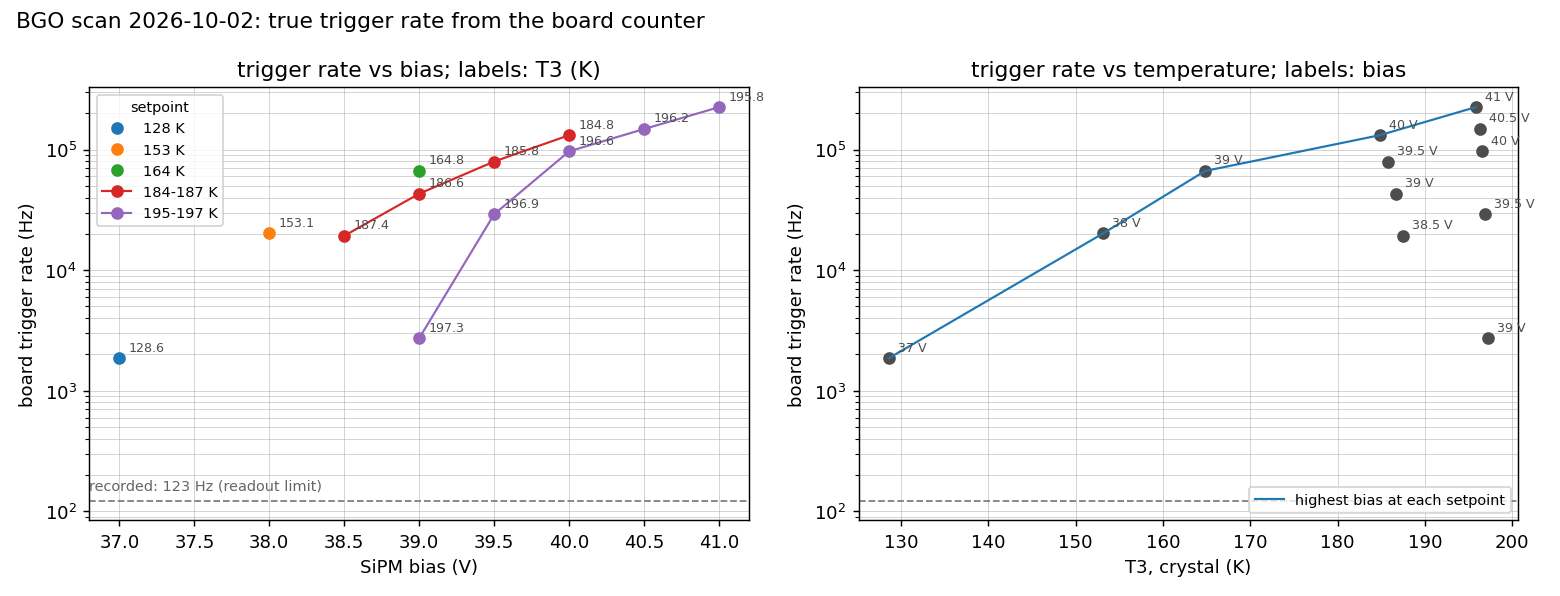
\includegraphics[width=\linewidth]{figs/scan_rates.png}
\caption{The true trigger rate of the board, from the trigger counter.
Left: against the bias, one colour per temperature setpoint, the two bias
scans joined by lines, each point labelled with its T3; the dashed line is
the recorded rate, the same in all runs. Right: against T3, each point
labelled with its bias; the line joins the five runs of the temperature
scan.}
\label{fig:rates}
\end{figure}

That it is the overvoltage and not the temperature that drives the rate
is seen at fixed bias. Three runs were taken at 39~V: the rate is 66~kHz at
165~K, 43~kHz at 187~K and 2.7~kHz at 197~K. The dark-count rate of a SiPM
grows with temperature, so at fixed overvoltage the rate would rise along
this sequence; it falls, because at fixed bias the overvoltage drops as
the breakdown voltage rises with the temperature, the gain drops with it,
and the single-photoelectron pulse falls below the threshold. The steepness
at 196~K, a factor 10 between 39 and 39.5~V, is the signature of the
threshold sitting close to the amplitude of one or two photoelectrons.

Two consequences follow. The recorded events are a random sample of the
triggers, from 7\% of them at 128~K to 0.05\% at 196~K and 41~V, so the
fraction of recorded events that contain a scintillation pulse is of the
order of the ratio of the real event rate to the trigger rate: most of them
at the cold end, and a few percent at the warm end at nominal bias. And
the trigger fires late on a real event, because a 511~keV pulse spreads
its photoelectrons over microseconds and few of them overlap in any
channel at any instant: a channel sees 7 to 13 counts at the peak against
a threshold of 19, and it crosses the threshold only when noise helps,
at a random time along the pulse. The start of the pulse is then often
before the record, or inside the 1.6~\us that precede the trigger.

\section{What the events look like}
\label{sec:events}

Figure~\ref{fig:event_channels} shows the 64 channels of one event of the
run at 197~K and 39~V, the raw counts of each channel minus its WebDump
baseline. The light is in a dozen channels: the row 48 to 55, and 11 and
12, each with a pulse of 10 to 25 counts rising at the trigger and decaying
over a microsecond. The other channels show the noise of the chain, 3.9
counts rms per sample, white except for a correlation between neighbouring
samples (Section~\ref{sec:spe}), and here and there an isolated spike of
about 15 counts, which is a dark pulse of one photoelectron.

\begin{figure}[tbp]
\centering
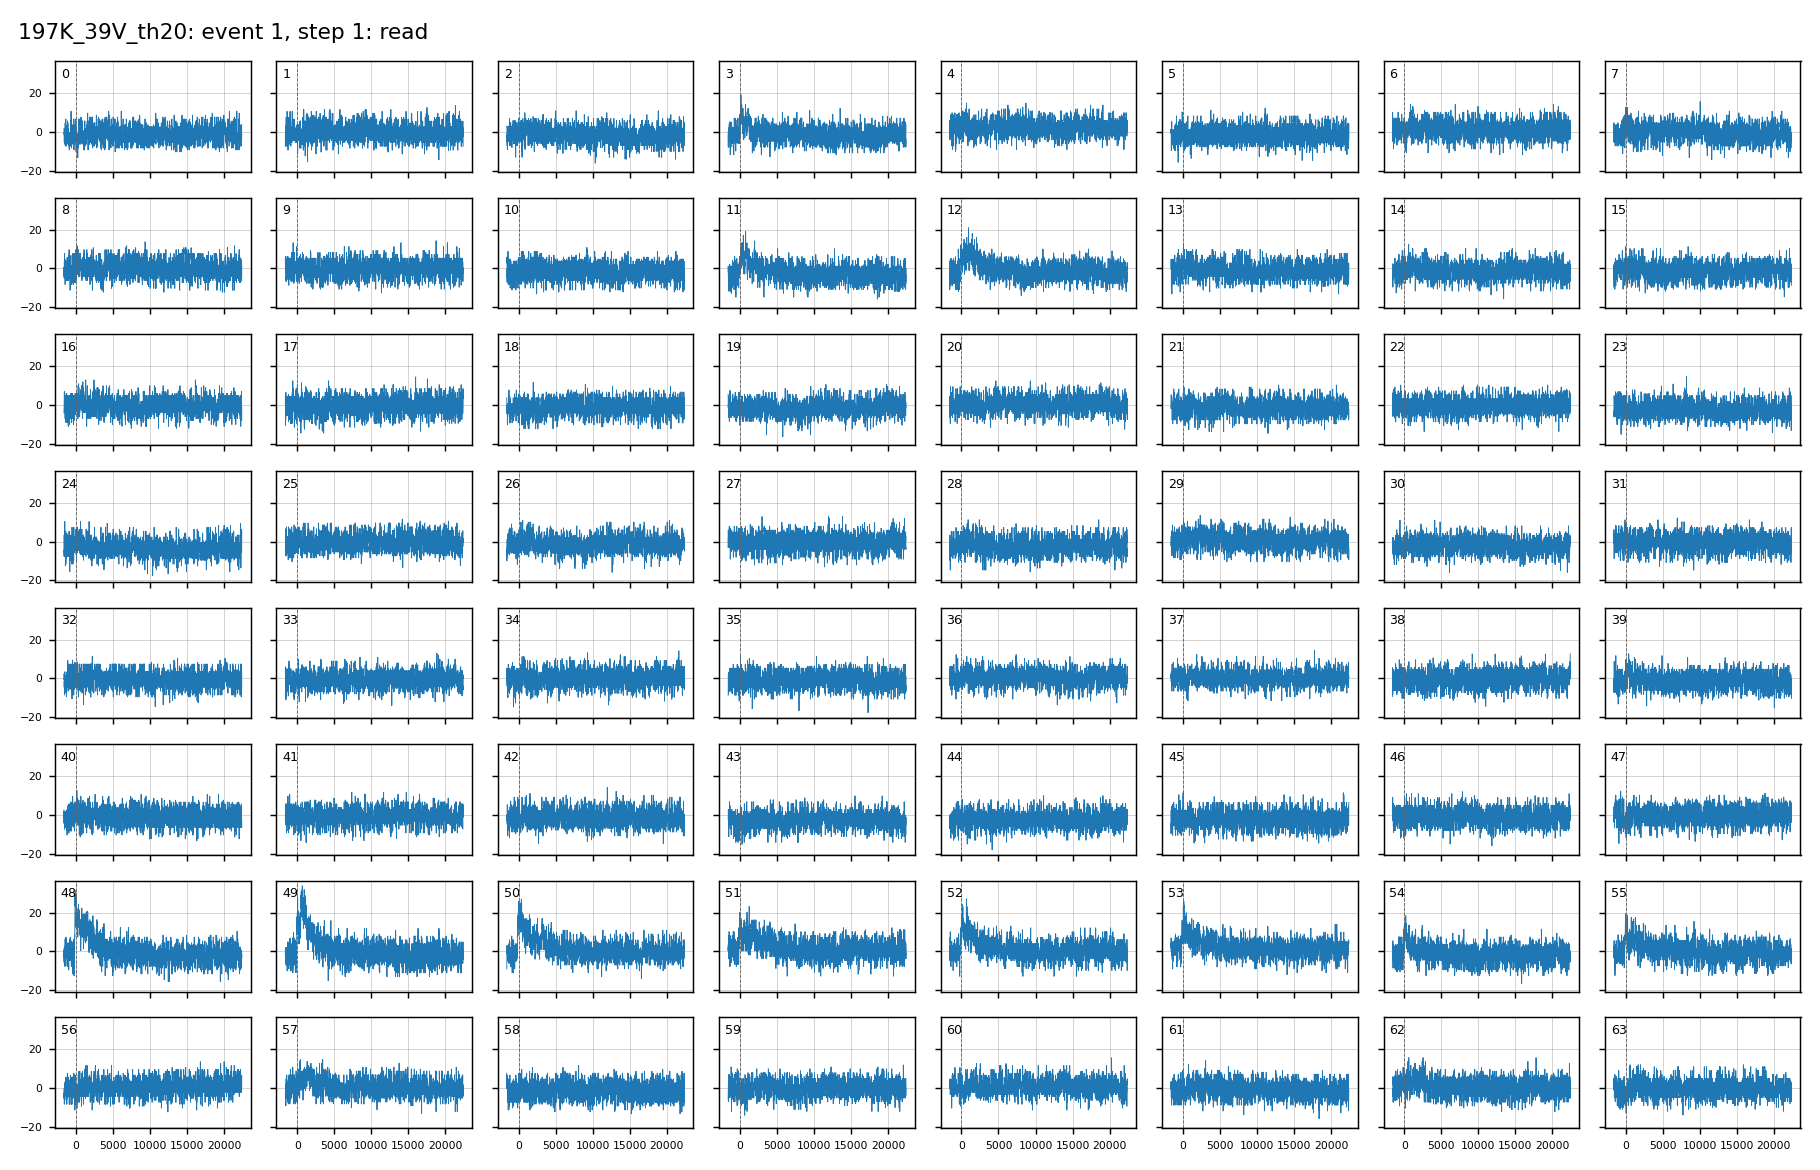
\includegraphics[width=\linewidth]{figs/sel_197K_ev1_s1.png}
\caption{Event 1 of \code{197K\_39V\_th20}: the 64 channels in channel order,
raw counts minus the WebDump baseline, against the time from the trigger
in ns. The light is in channels 48 to 55 and 11, 12.}
\label{fig:event_channels}
\end{figure}

Figure~\ref{fig:event_sum} shows the sum of the 64 channels of the same
event, after the correction described in the analysis note, with a moving
average over 64 samples (0.5~\us) on top. The pulse is 140 counts high
on the average, 200 on the raw sum, against 23 counts of noise per sample
in the sum; it rises at the trigger and decays in about 1~\us at this
temperature. At 128~K the decay is several microseconds long, and the
pulse is larger. The noise of the sum is what 64 channels of 3.9 counts add
up to, $3.9 \sqrt{64} = 31$, reduced by the correction: the part of the
noise that is common to all channels is small, 3\% of the variance of a
channel, and the sum is dominated by the independent white noise of the 64
channels.

\begin{figure}[tbp]
\centering
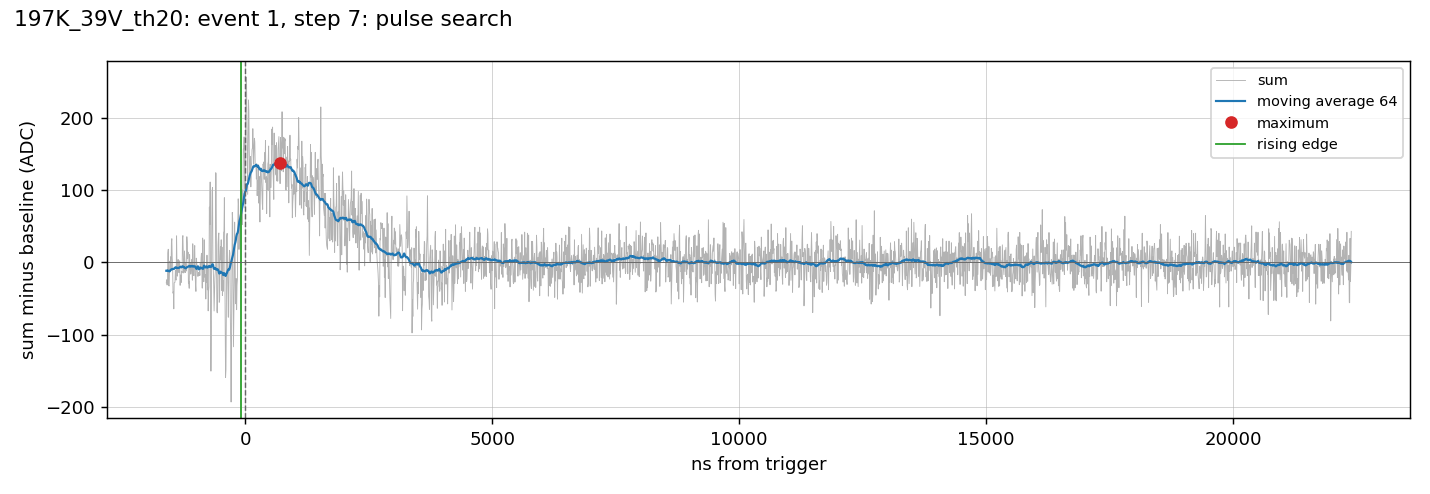
\includegraphics[width=\linewidth]{figs/sel_197K_ev1_s7.png}
\caption{The same event: the sum of the 64 channels, baseline subtracted
(grey), its moving average over 64 samples (blue), the maximum of the
average (dot) and the rising edge, where the average crosses half the
maximum (green line).}
\label{fig:event_sum}
\end{figure}

Three features of the events shape the analysis and are only named here.
The pre-trigger window is not free of signal, for the reason given in the
previous section, so the baseline of each event has to be taken from the
end of the record, 22~\us after the trigger, where the pulse is over. In
some events the pulse started before the record and only its tail was
recorded; these have to be recognised and set apart, and since small
pulses trigger later than large ones, they are lost preferentially, which
biases the spectrum. And with 24~\us of record and a real event rate of a
few kHz, a few percent of the records hold a second pulse, which has to be
found and flagged. The classification of the events, the choice of the
charge window and the definition of the charge are the first steps of the
analysis note.

\section{The 64 channels}
\label{sec:channels}

The channels are not all alike, and the single event of
Figure~\ref{fig:event_channels} already suggested it: the same channels,
48, 49, 11 and 12, carry the light in most of the events we looked at,
which a source that illuminates the whole crystal should not produce.
Figure~\ref{fig:chanstat} shows four maps of the channels accumulated over
500 events of the run at 195~K and 41~V: the noise of each channel in the
last 10~\us of its records, where there is no scintillation light; the
number of dark pulses above 20 counts found there; the fraction of events
in which the channel carries a significant charge in the scintillation
window (more than five times its own charge noise, measured in a control
window); and its mean charge when it does.

\begin{figure}[tbp]
\centering
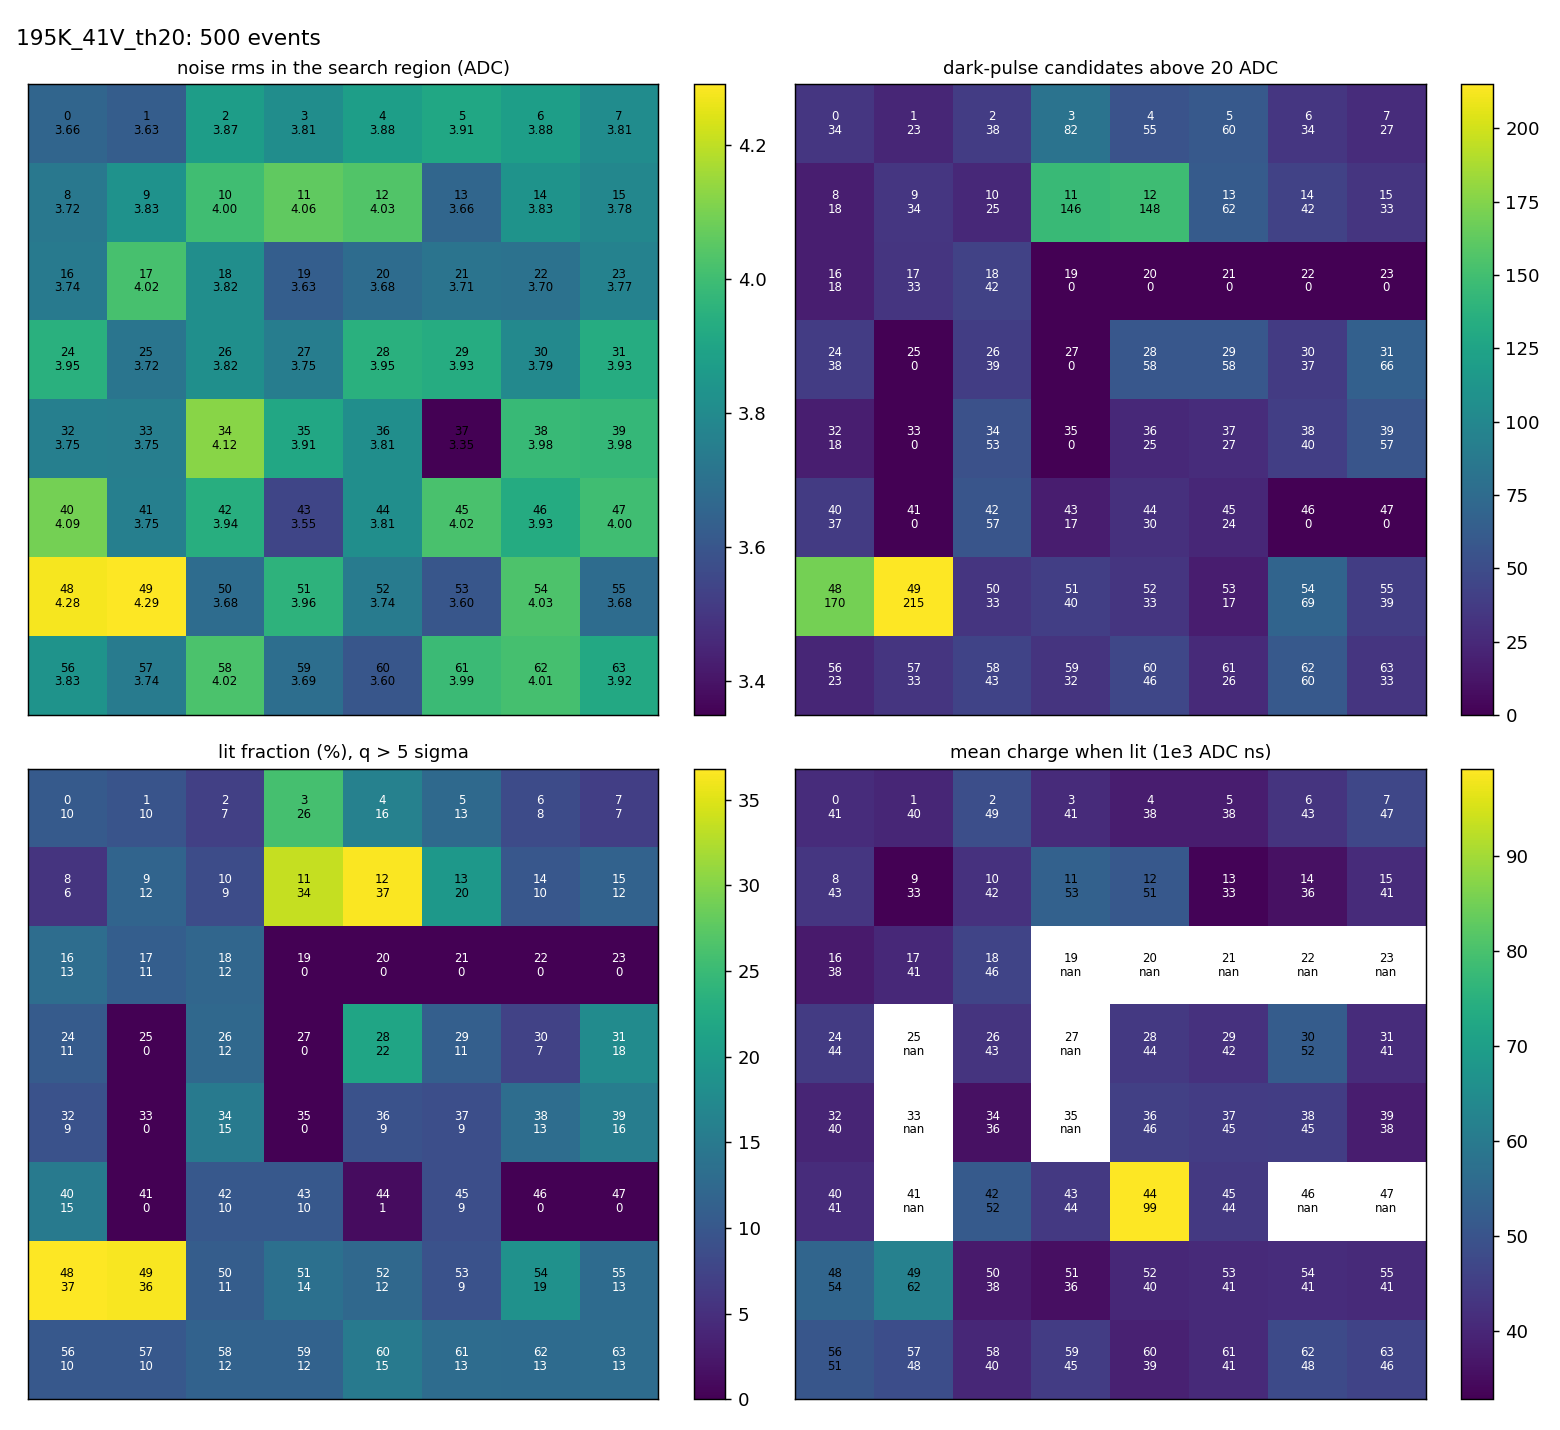
\includegraphics[width=\linewidth]{figs/chanstat_195K.png}
\caption{The 64 channels over 500 events of \code{195K\_41V\_th20}, in
channel order. Top left: noise rms per sample in the last 10~\us of the
record. Top right: dark pulses above 20 counts in the same region. Bottom
left: fraction of events in which the channel is lit, its charge in the
scintillation window above five times its charge noise. Bottom right: mean
charge when lit.}
\label{fig:chanstat}
\end{figure}

The noise is uniform, 3.4 to 4.3 counts rms, with no outlier. Everything
else is not.

Twelve channels are dead: 19 to 23, 25, 27, 33, 35, 41, 46 and 47. They
have the noise of every other channel, no dark pulse above 16 or 20 counts
in 20~ms of search time, a lit fraction of exactly zero in 500 events, and
a charge noise 30\% below the live channels, which is what pure white noise
gives when there are no pulses at all. They see no light and no dark
counts: no bias, or no connection. On the face they form a block, the
right five of the third row, two columns at the left of rows 4 to 6, and
two cells at the right of row 6, 19\% of the area. Light that falls on them
is lost. Whether these channels were known to be dead, and whether the
fault is in the SiPMs, the bias or the cables, is a question for the
people who took the data.

Four channels, 11, 12, 48 and 49, stand out the other way. Their noise is
at most 12\% above the median, so they are not noisy. They have five times
the dark pulses above 20 counts of the others, they are lit in 34 to 37\%
of the events against a median of 11\%, and when lit they carry 30 to
50\% more charge. One cause explains the four numbers: a larger gain.
Larger single photoelectrons cross a fixed threshold more often, the same
light gives more charge, and the channel passes a significance cut more
often. The recurring cluster at these channels is therefore a gain pattern,
not a position. Section~\ref{sec:spe} measures the gain and settles where
it comes from.

Channel 44 has normal noise and dark pulses but a charge noise three times
the others, and it is lit in 1\% of the events with twice the charge: its
baseline wanders slowly. It is kept with that caveat. The lit fraction of
the remaining 47 channels is flat across the face, 7 to 20\% with no edge
or row pattern: the source does illuminate the whole crystal, and at this
level the channel map shows nothing wrong, though the dead block hides part
of it.

\section{The single photoelectron}
\label{sec:spe}

The gain of a channel is the size of the pulse of one photoelectron. We
need it for three things: to put the 64 channels on the same scale before
summing them, to express the light yield in photoelectrons rather than in
counts, and, through its dependence on the bias, to measure the breakdown
voltage. There is no dedicated single-photoelectron run; the pulses have
to be found among the dark pulses in the part of the records that holds no
scintillation light, the last 10~\us.

\subsection{The pulse shape}

Figure~\ref{fig:template} shows the shape of the pulse, obtained from
13\,845 dark pulses of the run at 195~K and 41~V, where the pulses are
largest. The pulses were found as local maxima of the raw channel above 20
counts, a high threshold so that most of them are real, aligned on their
maximum sample, corrected for the local level by the median of the samples
before the peak, and averaged. The pulse rises in two samples, 16~ns, is
3.0 samples wide at half maximum, 24~ns, and decays over six samples,
50~ns. The same average from the first 300 events and from 2000 events
agrees to the third decimal. It carries a known defect: a pulse passes the
threshold more easily when the noise on its peak sample is positive, so
the central sample of the average is inflated, by about one count in
thirteen, and the shape is slightly too sharp. The normalised shape,
peak~1, is the template used below.

\begin{figure}[tbp]
\centering
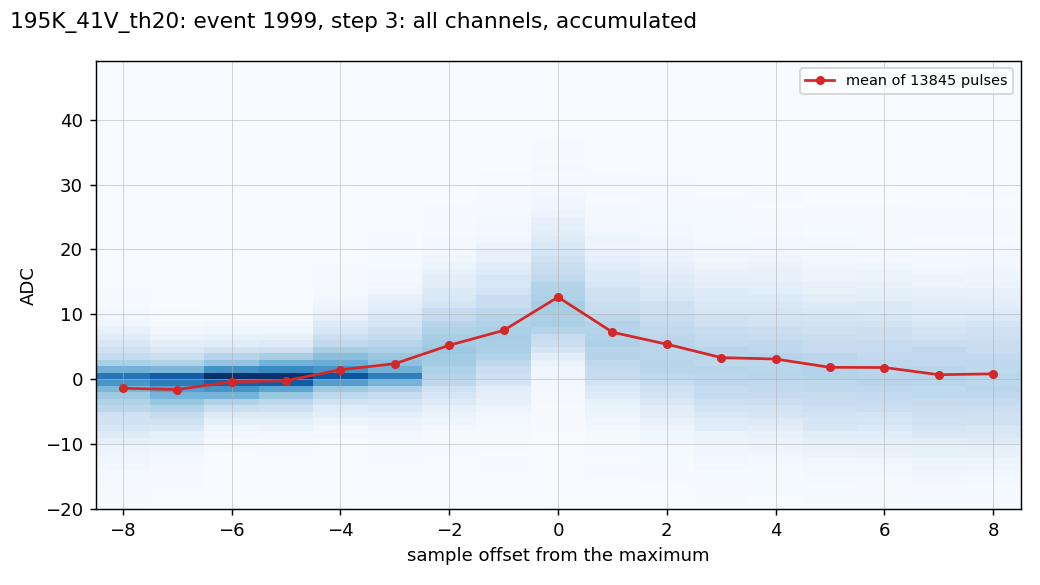
\includegraphics[width=0.75\linewidth]{figs/tpl_195K_s3.png}
\caption{The dark pulses of \code{195K\_41V\_th20} above 20 counts, aligned on
their maximum: the two-dimensional histogram of the amplitude against the
sample offset from the maximum, and the mean (points). The pre-peak samples
sit at zero after the local-level correction; the spread after the peak,
$\pm 10$ counts, is from pulses sitting on other pulses.}
\label{fig:template}
\end{figure}

\subsection{The noise, and why no filter helps}

A single photoelectron is 15 to 20 counts high on 3.9 counts of noise per
sample: a 4 to 5~sigma object if one looks at one sample. The standard
remedy is a matched filter, a weighted sum of consecutive samples with the
pulse shape as weights, which for white noise improves the signal to noise
by the square root of the sum of the squared weights, 1.5 for this pulse.
The dead channels, which hold nothing but noise, allowed us to measure the
noise rather than assume it (Figure~\ref{fig:noise}). It is correlated
between neighbouring samples, 0.43 at one lag and 0.16 at two, nothing
beyond, and its power spectrum is nearly flat up to the Nyquist frequency of
62.5~MHz, like the spectrum of the pulse itself: the pulse occupies the
same band as the noise. The matched filter then gains 1.09, and the best
linear filter for this noise, the matched filter applied after whitening,
gains 1.17; both predicted from the measured noise and verified on the dead
channels. There is no filter that makes the single photoelectron better
than a 5~sigma object at 41~V and a 4~sigma object at 39~V. This is a
property of the chain, 8~ns samples and a 24~ns pulse on 3.9 counts of
noise, and it limits what follows.

\begin{figure}[tbp]
\centering
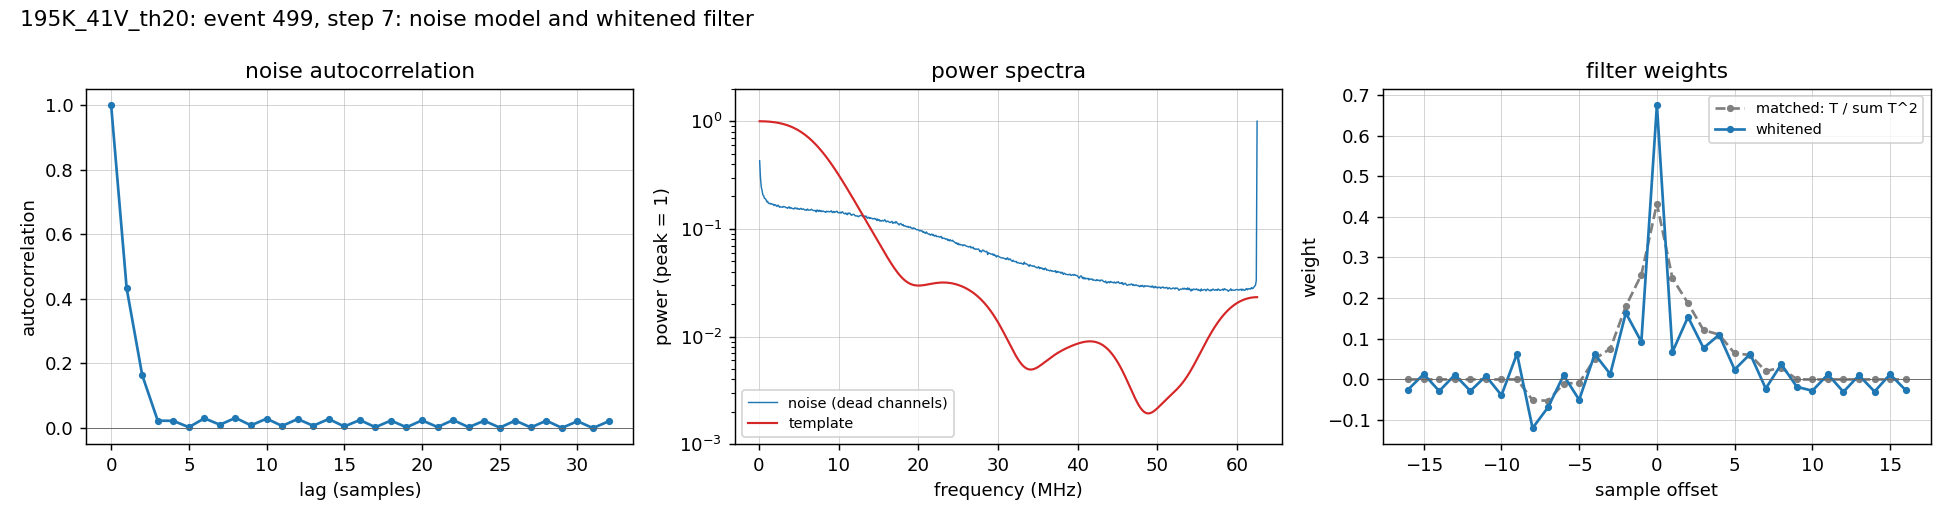
\includegraphics[width=\linewidth]{figs/tpl_195K_s7.png}
\caption{The noise of a channel, from 6000 segments of 10~\us of the
twelve dead channels. Left: autocorrelation against the lag in samples.
Centre: power spectrum, and the spectrum of the pulse template on the same
axis. Right: the weights of the matched filter and of the whitened filter
over a window of 33 samples.}
\label{fig:noise}
\end{figure}

\subsection{The spectra at 41 V and the equalization}

With the matched filter and a threshold at 4.5 times the filtered noise,
about 17 counts, the dark pulses of every channel of every event were
collected over the full run at 195~K and 41~V: 28\,664 candidates, 0.09
per channel and record, with the height of each one estimated by the
filter in counts of the raw peak. Figure~\ref{fig:spe} shows the spectrum
of the heights for one channel and for all live channels together, and
Figure~\ref{fig:spe_channels} the spectrum of every channel. In nearly
every live channel there is a peak at about 20 counts, cut on its low side
by the threshold, with a tail to the right from pulses with a crosstalk
partner and from overlapping pulses. The dead channels show only a spike
at the threshold, which is the contribution of noise maxima; it is a few
percent of the candidates of a live channel.

\begin{figure}[tbp]
\centering
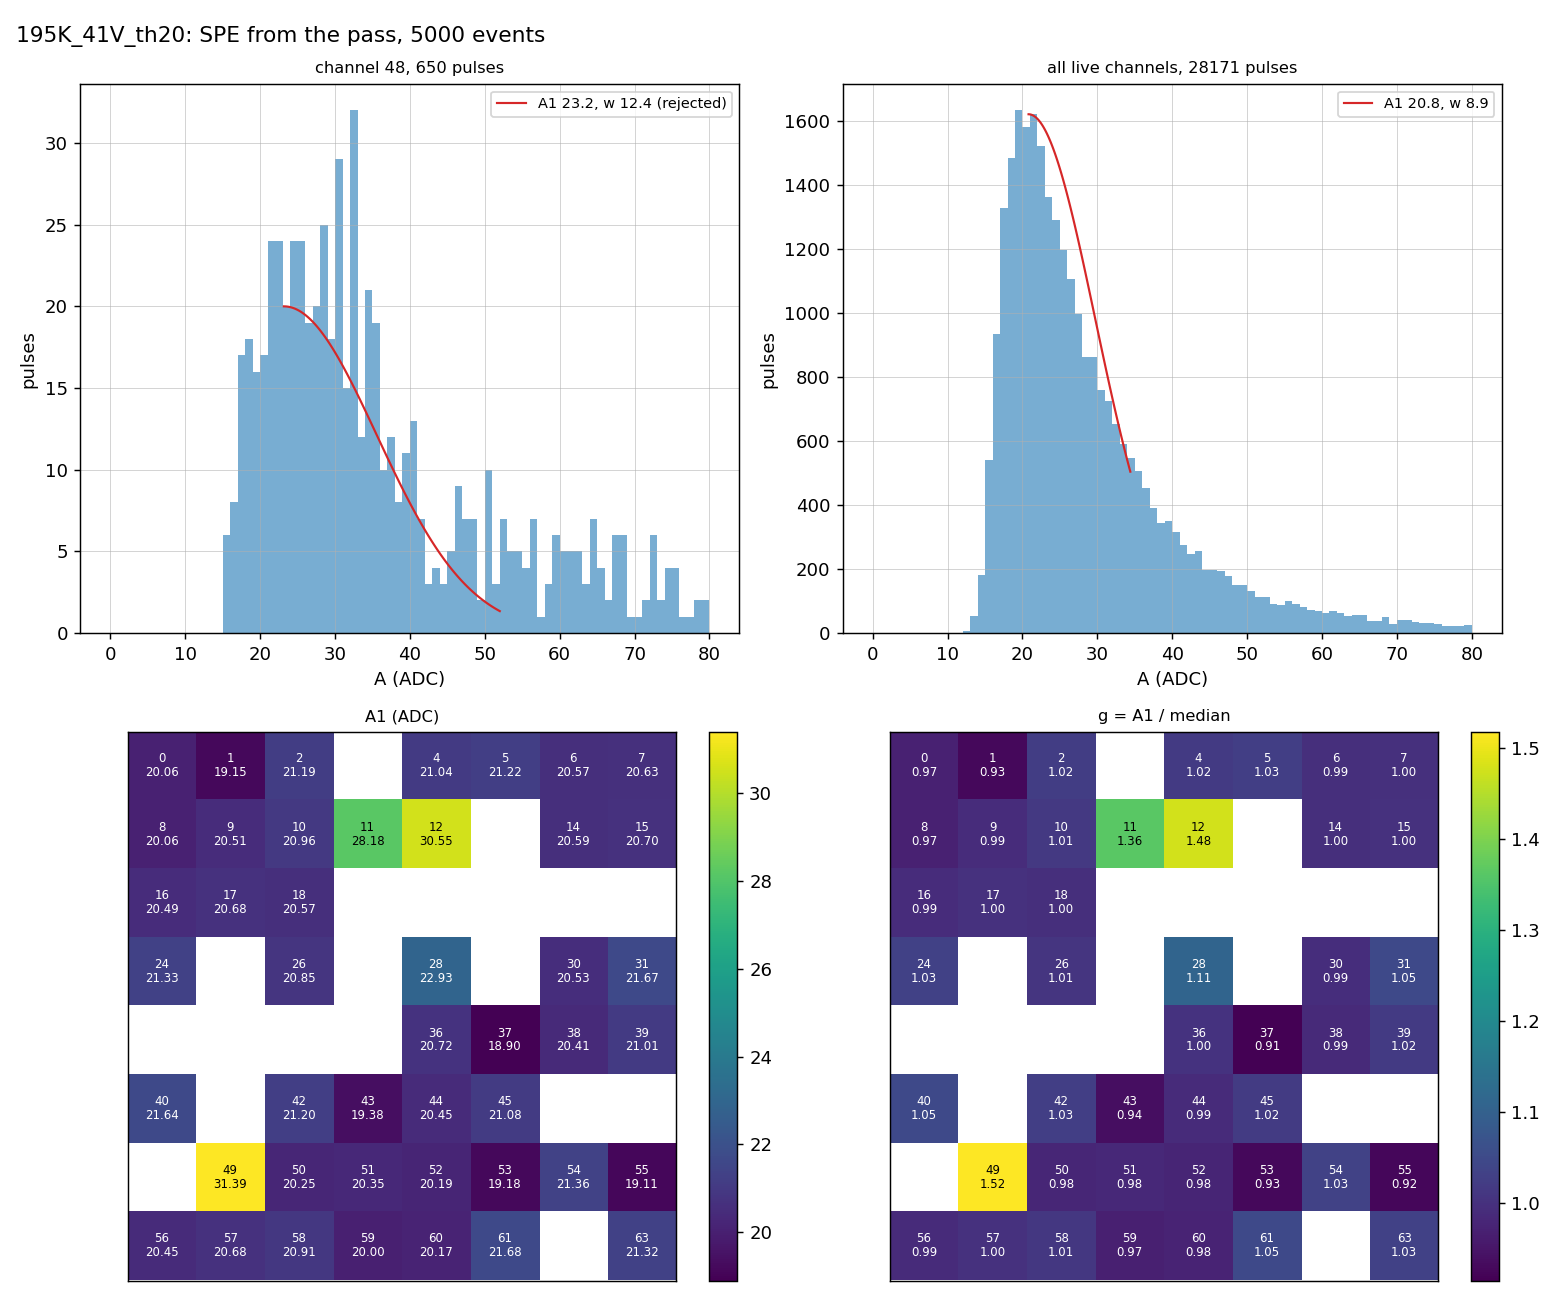
\includegraphics[width=\linewidth]{figs/spefit_195K.png}
\caption{Single-photoelectron spectra of \code{195K\_41V\_th20}, 5000 events.
Top left: channel 48. Top right: all live channels together, with the fit.
Bottom: the fitted amplitude $A_1$ per channel, and the equalization factor
$g_c = A_1 / 20.7$; empty cells are the dead channels and the channels
without an accepted fit.}
\label{fig:spe}
\end{figure}

\begin{figure}[tbp]
\centering
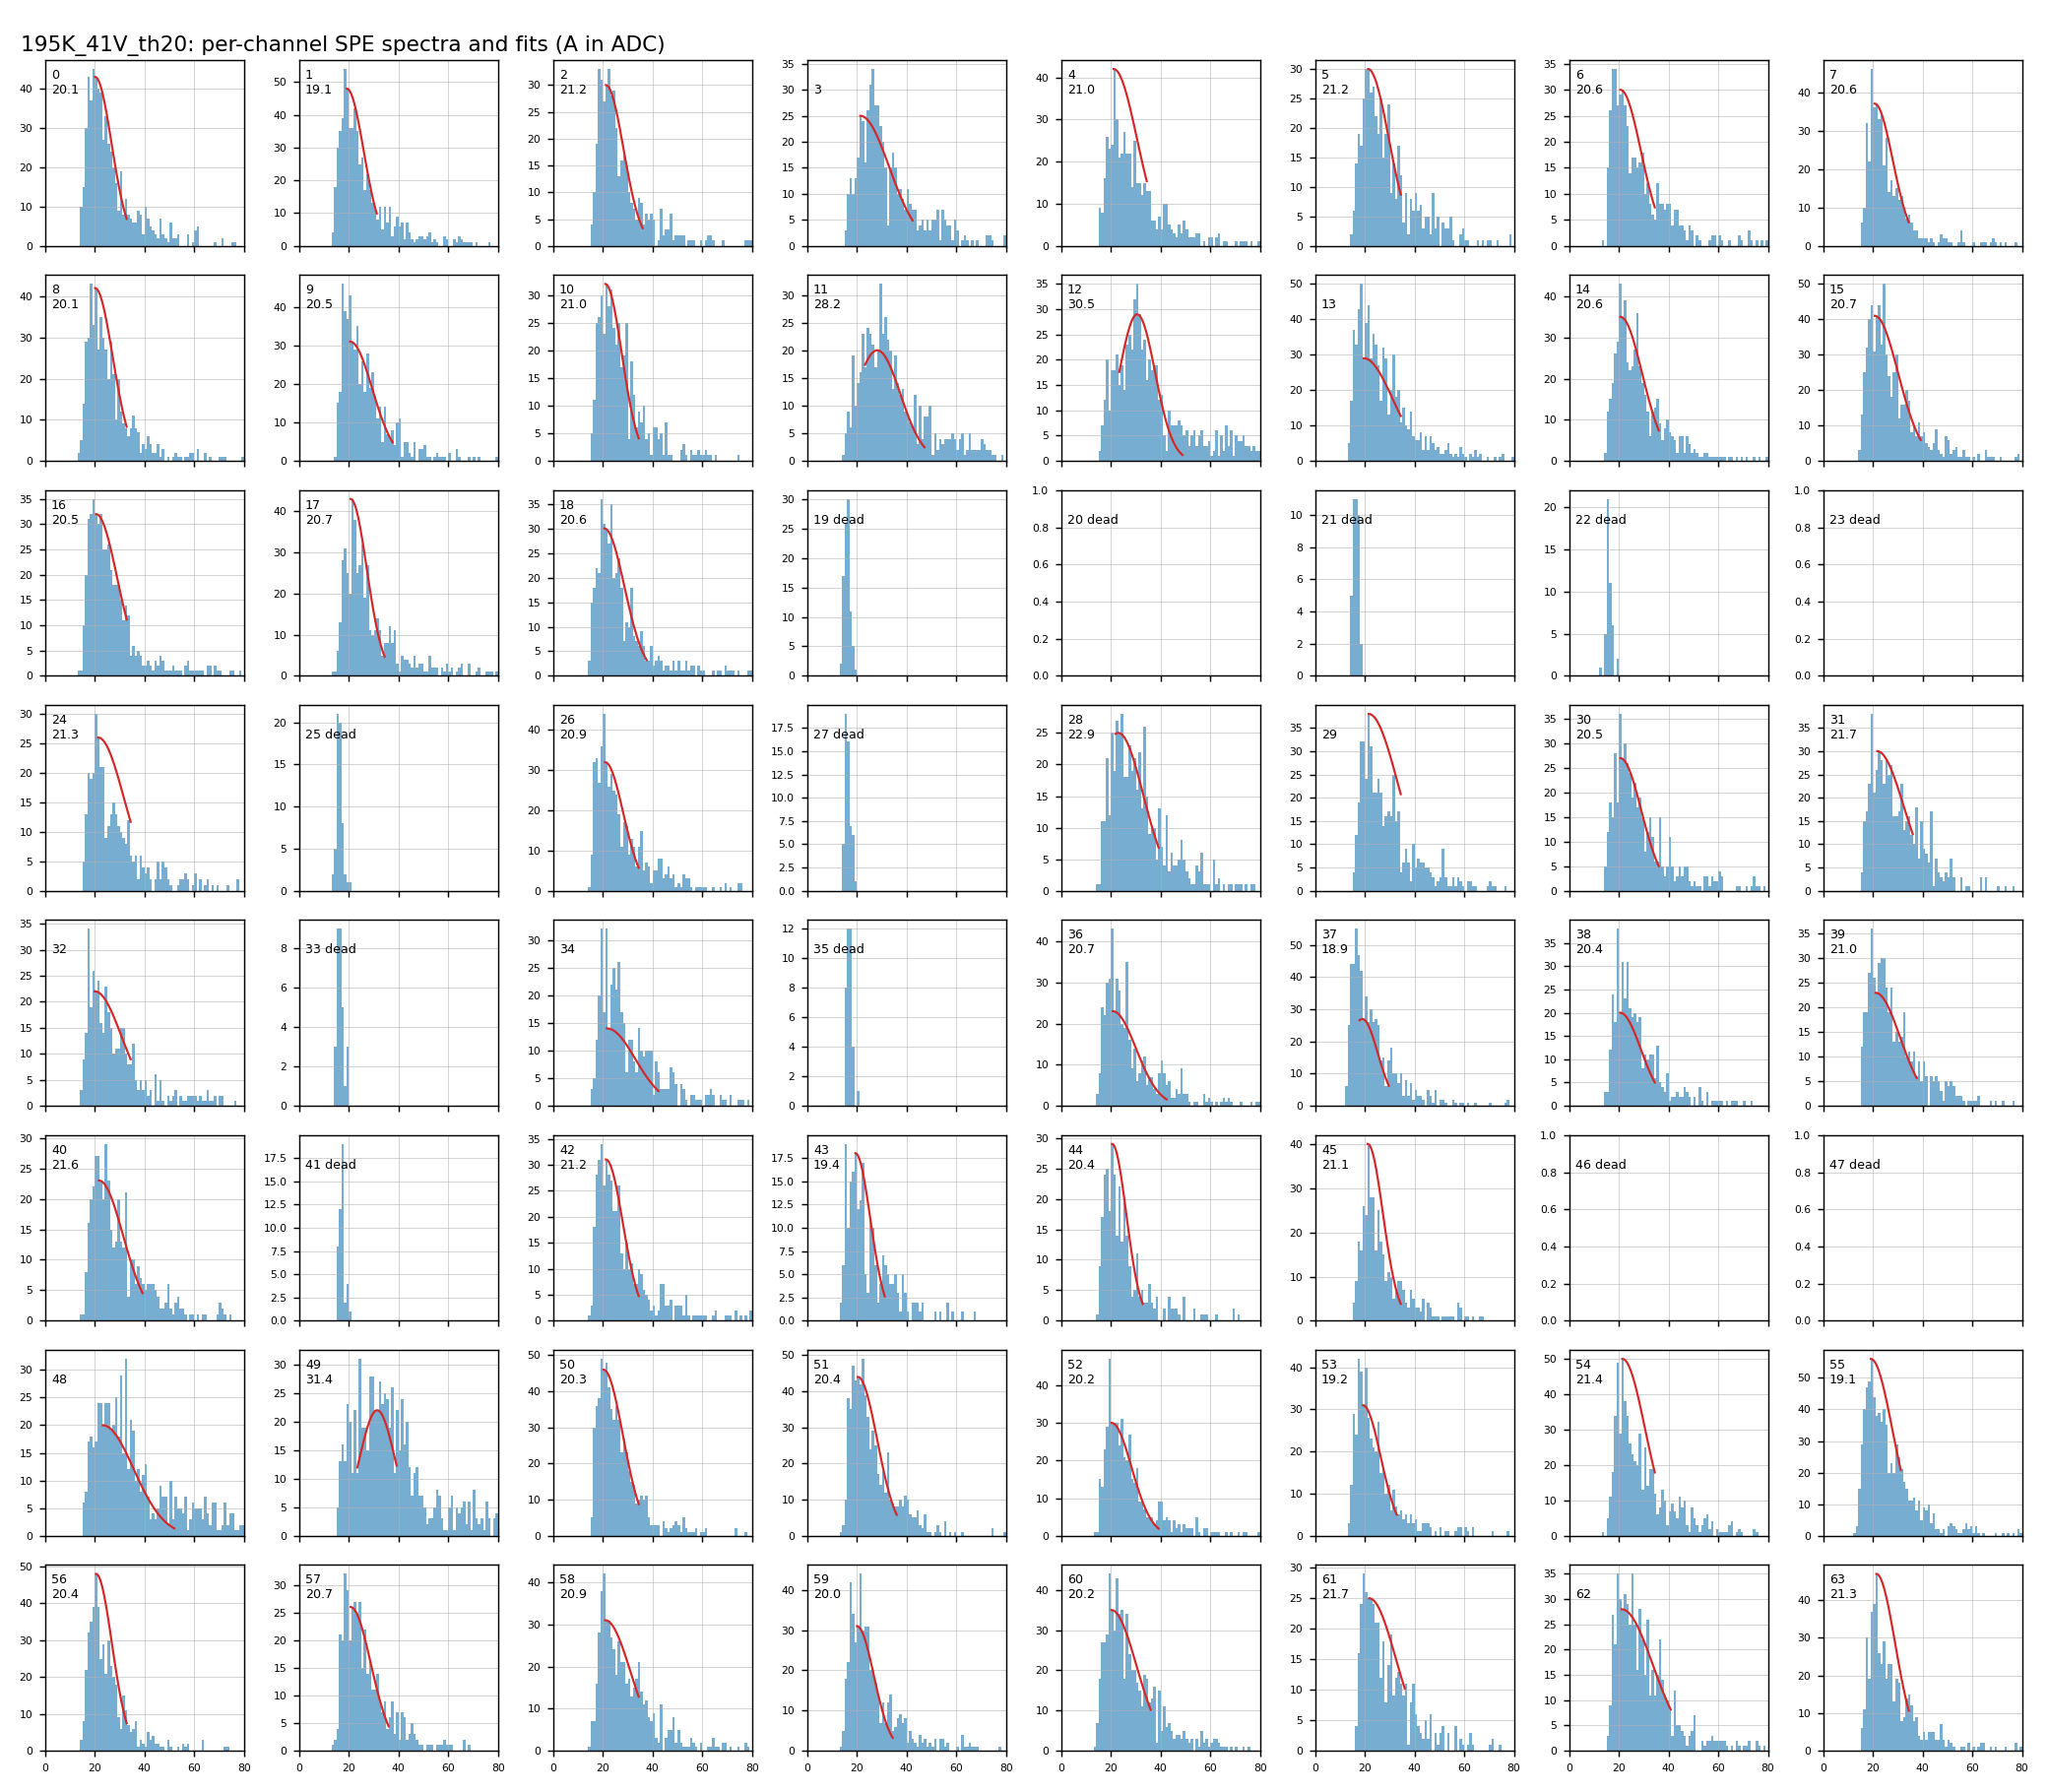
\includegraphics[width=\linewidth]{figs/spefit_195K_channels.png}
\caption{The spectrum of every channel, same run, with the fitted Gaussian
where the fit was accepted and $A_1$ in the corner. The dead channels show
only the spike at the threshold.}
\label{fig:spe_channels}
\end{figure}

The peak of each channel was fitted with a Gaussian from one noise width
above the threshold to 1.6 times the mode (fitting from the threshold
itself was tried; the Gaussian then stretches over the truncation and the
fit is worse). Forty-five of the 52 live channels give an accepted fit. The
median of the fitted amplitudes is 20.7 counts, and the normal channels
lie within $\pm 9\%$ of it, with errors of 1 to 4 counts each, which come
from the peak sitting only one noise width above the cut. The four
channels of Section~\ref{sec:channels} are where they were expected: 11 at
$28.2 \pm 1.5$ counts, 12 at $30.5 \pm 0.6$, 49 at $31.4 \pm 0.7$, that is
1.36, 1.48 and 1.52 times the median. Channel 48 has two populations, one
at the normal 22 counts and one at 33, and no single peak to fit; its gain
will have to come from its response to the scintillation light. The dark
rate of the live channels, from the number of candidates and the search
time, is 8 to 15~kHz at this overvoltage.

The equalization factor of a channel is $g_c = A_1(c) / 20.7$, and the
table of the 45 factors is in \code{src/spe\_gain\_195K\_41V\_th20.csv}.
Dividing each channel by its factor before summing puts the 64 channels in
the units of the median channel.

\subsection{The bias scan: breakdown voltage, and the nature of the four channels}

The same collection and fit were done on the other four runs of the bias
scan at 196~K, at 40.5, 40, 39.5 and 39~V. For the normal channels the
result is not a measurement: the number of candidates falls from 28\,664
at 41~V to 2705 at 39~V, while the fitted amplitude stays at 20 to 21
counts whatever the bias. The true peak slides down with the overvoltage,
from 20.7 counts to about 14 at 39~V, below the 17-count threshold, and
what the fit sees is the remnant above the cut, pinned just above it. The
normal channels can be followed only at 41~V.

The four high-gain channels can be followed further, because their peak
stays above the cut. Channel 49, the cleanest, gives $31.4 \pm 0.7$,
$29.2 \pm 1.5$ and $26.7 \pm 2.3$ counts at 41, 40.5 and 40~V: a slope of
4.7 counts per volt, which extrapolates to zero at 34.3~V. That is the
breakdown voltage of this SiPM at the temperature of the run. The datasheet
line gives 34.5~V at T3 and 34.9~V at T2, so the breakdown at 196~K is
where the extrapolation from the datasheet puts it, within half a volt,
and the data cannot tell whether the SiPMs were at the crystal temperature
or at that of the frame, as expected from the 0.3~V that separates the two
hypotheses.

The slope also says what the four channels are. If their larger gain came
from a lower breakdown voltage, their excess over the normal channels
would grow as the bias is lowered, since the ratio $(V - V_{\rm bd}^{\rm
ringer}) / (V - V_{\rm bd}^{\rm normal})$ grows as $V$ approaches the normal
breakdown. Dividing the amplitude of channel 49 by the normal amplitude
scaled with the overvoltage, $20.7\,(V - 34.5) / 6.5$, gives 1.52, 1.53,
1.53 and 1.48 at 41, 40.5, 40 and 39.5~V: constant. A constant factor is a
larger gain after the SiPM, in the shaper of that channel. The same holds
for 11 and 12 within their larger errors. The practical consequence is
welcome: the equalization factors do not depend on the bias or the
temperature, and the table from the 41~V run applies to every run,
including the cold ones where no dark pulse can be seen.

What this leaves open is stated plainly. The single-photoelectron
amplitude of the normal channels is measured at one point, 41~V and 196~K,
and the gain of every other run has to come from the datasheet dependence
of the gain on the overvoltage, anchored at that point and checked by the
light itself: the position of the 511~keV photopeak along the bias scans
is the next measurement of the same quantity, and it is where the analysis
note begins.

\end{document}
